
\documentclass[11pt]{article}

%\setlength\topmargin{-0.1in}
%\setlength\headheight{0in}
%\setlength\headsep{0in}
\setlength\textheight{8.5in}
\setlength\textwidth{6.5in}
\setlength\oddsidemargin{0in}
\setlength\evensidemargin{0in}
\setlength{\parindent}{0pt}
\usepackage{placeins}
%\usepackage{indentfirst}

\usepackage{amsmath}
\usepackage{graphicx}
\usepackage{listings}
\usepackage{rotating}
\usepackage{subcaption} 
\usepackage{booktabs}
\usepackage{tikz}
\usepackage{fancyhdr}
\usepackage{pdfpages}
\usepackage{hyperref}
\usepackage{longtable}
\usepackage[toc,page]{appendix}
%For The 2x2 Figure
\usepackage{subcaption}
\usepackage{mwe}
% To import matlab code
\usepackage{listings}
\usepackage{matlab-prettifier}
\usepackage[framed,numbered,autolinebreaks,useliterate]{mcode}
%Glossary
\usepackage[acronym,nonumberlist]{glossaries}
%\glsaddall %includes all acronymns
%Tables
\usepackage{booktabs}
\newcommand{\ra}[1]{\renewcommand{\arraystretch}{#1}}
%Nomenclature
\usepackage{nomencl}
\makenomenclature
\newif\iffirstglossary\firstglossarytrue
%% This removes the main title:
\renewcommand{\nomname}{}
%% this modifies item separation:
\setlength{\nomitemsep}{15pt}
%% this part defines the groups:
%----------------------------------------------
\usepackage{etoolbox}
\renewcommand\nomgroup[1]{%
  \item[\Large\bfseries
  \ifstrequal{#1}{N}{Nomenclature}{%
  \ifstrequal{#1}{A}{List of Abbreviations}{}}%
]\vspace{10pt}} % this is to add vertical space between the groups.
%----------------------------------------------



\pagestyle{fancy}
\usetikzlibrary{shapes,arrows}
\graphicspath{{Figures/}}
\newcommand{\tabitem}{~~\llap{\textbullet}~~}

\newcommand*{\MyIndent}{\hspace*{0.5cm}}%inerts tab in tables



 
\begin{document} 
\pagenumbering{gobble}

	\begin{titlepage}
	\thispagestyle{empty}
		\newcommand{\HRule}{\rule{\linewidth}{0.5mm}}	
		\center
		\LARGE 
		University of Bath\\
	 	Faculty of Engineering \& Design\\[1cm]	
		%textbf{\Large ME30313 Group Business & Design}\\
		\large
		Word count: 2154\\[0.5cm]
		{\large\today}\\[1cm]	
		\HRule\\[0.4cm]	
		{\LARGE \bfseries Advanced Helicopter Dynamics}\\[0.3cm] 	
		\HRule\\[1cm]	
		\begin{minipage}{0.4\textwidth}
			\begin{flushleft}
				\large
				\textit{Supervisor}\\
				D. \textsc{Cleaver}
			\end{flushleft}
		\end{minipage}
		~
		\begin{minipage}{0.4\textwidth}
			\begin{flushright}
				\large
				\textit{Assessor}\\
				
			\end{flushright}
		\end{minipage}\\[1.4cm]
		\large
		\textit{Author's Candidate Number}\\
		10838\\
		\vfill
		\includegraphics[width=0.4\textwidth]{UOB_Logo.png}\\
		\vfill 
	\end{titlepage}

%%% ACRONYMS %%

%%END OF ACRONYMS %%%


\thispagestyle{empty}




\tableofcontents
\thispagestyle{empty}
\listoffigures
\listoftables

\nomenclature[A]{BEMT}{Blade Element Momentum Theory}


%\printnomenclature


\clearpage
\pagenumbering{arabic}
%\setcounter{page}{1}
\section{Introduction}

Somewhat surprisingly over the period of 2010 to 2017 total electricity generation in the United Kingdom fell by 18 \% \cite{data1} as consumption also fell 10\% across the period \cite{data2}. This is in spite of a rising population and number of households. This has been attributed to warmer winter lowering electric heating demands as well as improvements in refrigerator technology and increased use of LED lights \cite{guardian}. Using data made available by the UK Department for Business, Energy \& Industrial Strategy \cite{data1} it can be seen that wind power has defied the slowdown of electricity generation in the UK, rising an average 29\% year on year over the same 2010 to 2017 period. 

\begin{figure}[ht] 
        \centering
        \begin{subfigure}[b]{0.475\textwidth}
            \centering
            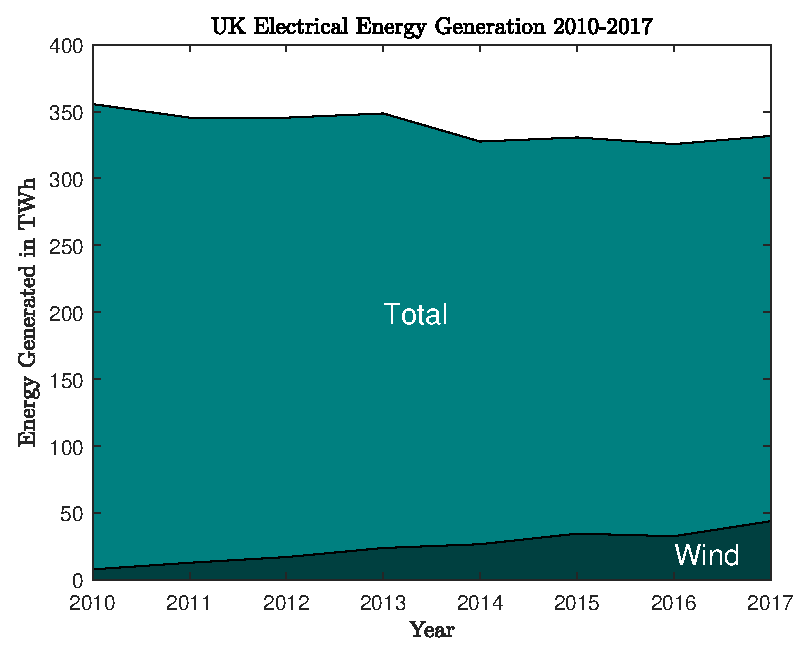
\includegraphics[width=\textwidth]{ukGen}
            \caption[Network2]%
            {{\small Annual Electrical Energy Generation }}    
            \label{fig:zoommesh1}
        \end{subfigure}
        \hfill
        \begin{subfigure}[b]{0.475\textwidth}  
            \centering 
            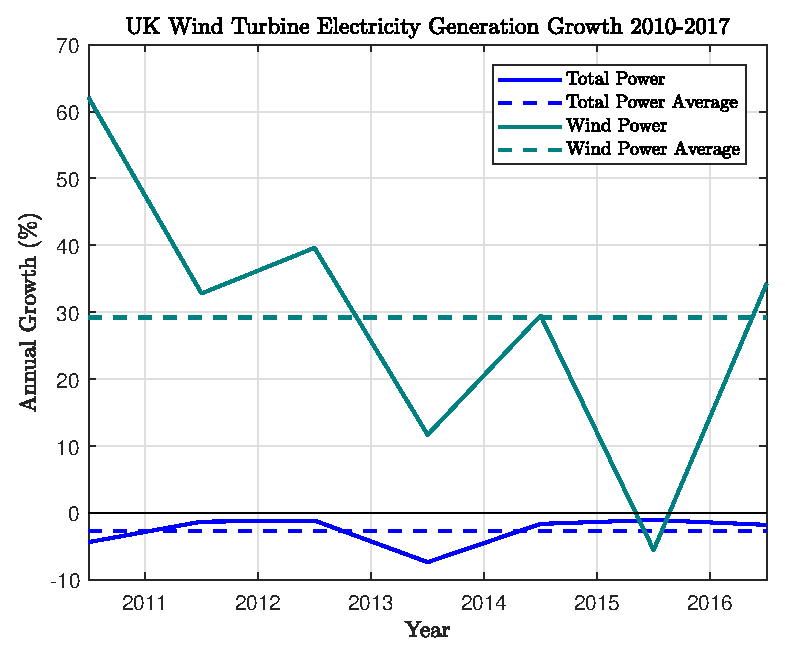
\includegraphics[width=\textwidth]{WindGrowth}
            \caption[]%
            {{\small Annual Growth of Electrical Energy Generation  }}    
            \label{fig:WindGrowth}
        \end{subfigure}
        \caption[ The Effect of Mesh Size on Temperature Resolution ]
        {\small Statistics on UK Electrical Energy Generation} 
        \label{fig:ukenergy}
    \end{figure}

Traditionally the wind sectors growth was completely reliant on large government subsidies but in recent years governments such as the UK and Germany have adopted a new approach to subsidisation which has lead to significant shift in the sector's economics. The government policy change was to make energy companies bid for projects and associated subsidies meaning the actual subsidy received is the difference between the subsidy and the bid. This competitive approach (contract for difference) has driven innovation with off-shore wind cost more than halving in the UK in just three years \cite{FT}. In some cases large wind projects have become viable with no subsidy or tax-break at all. The significance is the rate of development within the wind energy sector is now not reliant on government renewable energy policy but is shifting to large scale private sector investment. Due to the sheer size of the energy industry this could lead to significant wind turbine technology development. With the age of the electric car expected to dramatically reverse the trend of falling electricity consumption seen in Figure \ref{fig:WindGrowth}, research into wind turbine design has never been more relevant. \\

The optimal design of a wind turbine blade is one which produces the most power for the lowest unit cost \cite{handout}. This is would require a vast amount of cost data which is not readily available and so this paper shall instead focus on the design of a technically optimal design. Specifically the design which has the highest annual energy production (AEP) within the parameters given in Table \ref{table:parameters}. 


\begin{table}
	\centering
	\caption{Design Parameters for Wind Turbine Design \cite{handout}}
	\label{table:parameters}
	\includegraphics[width = 0.8\linewidth]{ParameterTable}
\end{table}

\FloatBarrier

\section{Methodology}

To find the optimal design blade element momentum theory was used to calculate power output for a given velocity and parameter set. Using Weibull's wind speed distribution and power output for a given velocity, AEP was calculated. Part A of the flow diagram of Figure \ref{fig:handoutflow} shows the flow of information for the computer program used to calculate the AEP.\\

\begin{figure}[h!]
	\includegraphics[width=0.75\textwidth]{HandoutFlow}
	\caption{Flow Diagram of Method Used to Find Annual Energy Production for the Turbine Design \cite{handout}}\label{fig:handoutflow}
\end{figure}

The design parameter's which could be changed for blade design were inclination at root: $\theta_0$, rate of twist: $\theta_{tw}$ and chord gradient: $c_g$. The theoretical maximum power output for a given wind speed, $V_0$, and reference area, A, is the called the Betz limit and is given by equation \ref{eq:betz}. The maximum theoretical AEP can be found using the Weibull distribution and the Betz limit. Using a minimum finding function from Matlab's library the combination of the three parameters which gives the least difference to the Betz limit AEP can be found thus finding the optimal design for the given parameter set.

\begin{equation}
	\label{eq:betz}
	P_{Betz} = \frac{16}{27} \left ( \frac{1}{2} \rho V_0^3 A \right )
\end{equation}
\FloatBarrier


\section{Results and Discussion}



\subsection{A: Optimal Design}
\subsection{B: Limitations of Model}
\section{Conclusions}










\begin{thebibliography}{9}
%Last name, First Initial, Year published. Title. Publisher, Volume, Page(s).
% HARVARD REFERENCE STYLE:
%Brunner, F.H., 1949. Synthetic gasoline from natural gas. Industrial and engineering chemistry, 41(11), pp.2511-2515.

\bibitem{data1} 
Department for Business, Energy \& Industrial Stratergy, 2018. 
\textit{Historical Electricity Data:1920 to 2017.}\\
Available: www.gov.uk/government/statistical-data-sets/historical-electricity-data

\bibitem{data2} 
Digest of United Kingdom Energy Statistics (DUKES), 2018. 
\textit{Digest of UK Energy Statistics (DUKES): electricity.}
Available:https://www.gov.uk/government/collections/electricity-statistics

\bibitem{moodleslides} 
Cleaver, D., 2018. 
\textit{Slides: WT Coursework.}\\
University of Bath.

\bibitem{handout} 
Cleaver, D., 2018. 
\textit{ME40343 Helicopter Dynamics: Coursework.}\\
University of Bath.

\bibitem{guardian} 
Vaughan, A., 2017. 
\textit{Electric cars will fuel huge demand for power, says National Grid.}\\
The Guardian.

\bibitem{FT}
Arie, S., 2018. 
\textit{Renewables are primed to enter the global energy race.}\\
The Financial Times.
\end{thebibliography}

\pagebreak

\begin{appendices}

%%AAAAAAAAAAAAAAAAAAAAAAAAAA%%%%%%%
\section{Induced Calculations Function}\label{ap:induced}

\lstinputlisting[style=Matlab-editor]{C:/Users/xav_m/OneDrive/Documents/XAVI/University/Final_Year/HELICOPTERS/Coursework/Windturbine_Optimisation/WTInducedCalcs.m}

\section{Wind Turbine Single Velocity Function}\label{ap:single}
\lstinputlisting[style=Matlab-editor]{C:/Users/xav_m/OneDrive/Documents/XAVI/University/Final_Year/HELICOPTERS/Coursework/Windturbine_Optimisation/WTSingleVelocity.m}

\section{Wind Turbine Velocity Range Function}\label{ap:range}
\lstinputlisting[style=Matlab-editor]{C:/Users/xav_m/OneDrive/Documents/XAVI/University/Final_Year/HELICOPTERS/Coursework/Windturbine_Optimisation/WTVelocityRange.m}

\section{Wind Turbine Velocity Range Function}\label{ap:optimisation}
\lstinputlisting[style=Matlab-editor]{C:/Users/xav_m/OneDrive/Documents/XAVI/University/Final_Year/HELICOPTERS/Coursework/Windturbine_Optimisation/TurbineOptimisation.m}

\section{Flow Chart of FEM Solver}
%\begin{lstlisting}
%function [SqMatrix] = LaplaceElemMatrix(D, eID, msh)
%
%%Returns the local 2x2 element matrix of a given element for a given diffusion
%%coefficient
%%
%% Inputs: 
%% D - Coefficient of Diffusion
%% eID - Index of element within mesh structure
%% msh - Mesh which contains local elements within it's structure
%
%%% Form of Laplace Elem matrix for J=1, D=1
%
%SqMatrix = [0.5, -0.5; ...
%            -0.5, 0.5];
%
%%% Multiply  by (1/J) and D to get solution for the particular element
%
%J = msh.elem(eID).J;  %Get Jacobi for the element
%
%SqMatrix = (1/J) * D * SqMatrix;   %Local element matrix for element eID
%end
%\end{lstlisting}
%\pagebreak










\end{appendices}





\end{document}

